У даному розділі досліджено плоска статична задача теорії пружності для прямокутної області,
за умов другої основної задачі теорії пружності на бічних гранях.

Вихідна задача зведена до одновимірної задачі у просторі трансформант за допомогою інтегрального перетворення Фур'є.
Отримана крайова задача розв'язана точно за допомогою методу матрично диференціального числення,
фундаментальний розв'язок представлений як інтеграл по замкненому контору, який в свою чергу, був знайденний за допомогою теоремі про лишки.
Остаточний вигляд для функцій переміщеннь та напружень отриман шляхом оберненого перетворення Фур'є.
Побудовано та розв'язано сінгульрне інтегральне рівняння відносно невідомої функції шляхом викорстання методу ортагональних поліномів, та зведення рівнняння до бескінечної алгебричної системи,
яка в подальшому була розв'язана методом редукціі.

Проведено чисельний аналіз отриманих функцій переміщень та напружень для різних розмірів прямокутної області та різних видів навантаження.

\subsection{Постановка задачі}
\begin{figure}[ht!]
    \begin{center}
        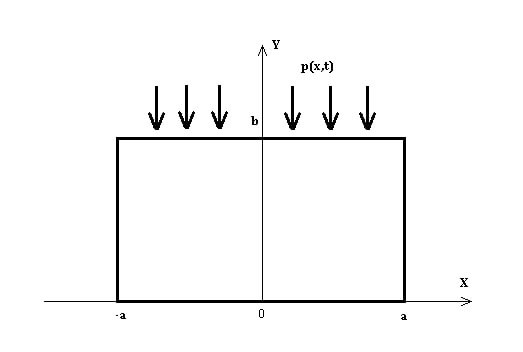
\includegraphics[scale=1]{images/geometry/image_1.jpg}
    \end{center}
    \caption{Геометрія проблеми}\label{geom_static_2}
\end{figure}
Розглядається пружна прямокутна область (Рис: \ref{geom_static_2}), яка займає облась,
що описується у декартовій системі координат співвідношенням $-a \le x \le a$, $0 \le y \le b$.

До прямокутної області на грані $y=b$ додане нормальне навантаження
\begin{equation}
    \sigma_y(x, y) |_{y=b} = -p(x), \quad  \tau_{xy}(x,y) |_{y=b} =0
\end{equation}
де $p(x)$ відома функція.

На бічних гранях виконується умова другої основної задачі теорії пружності
\begin{equation}
    u(x,y) |_{x=\pm a} = 0, \quad v(x,y) |_{x=\pm a} =0
\end{equation}
На нижній грані виконуються наступні умови
\begin{equation}
    v(x,y) |_{y=0} = 0, \quad \tau_{xy}(x,y) |_{y=0} =0
\end{equation}
Розглядаються наступні рівняння рівноваги Ламе:
\begin{equation}\label{lame_static_2}
    \begin{cases}
        \frac{\partial^2 u(x,y)}{\partial x^2} + \frac{\partial^2 u(x,y)}{\partial y^2} + \mu_0 (\frac{\partial^2 u(x,y)}{\partial x^2} + \frac{\partial^2 v(x,y)}{\partial x\partial y}) = 0 \\
        \frac{\partial^2 v(x,y)}{\partial x^2} + \frac{\partial^2 v(x,y)}{\partial y^2} + \mu_0 (\frac{\partial^2 u(x,y)}{\partial x \partial y} + \frac{\partial^2 v(x,y)}{\partial y^2}) = 0 \\
    \end{cases}
\end{equation}
Щоб розв'язати поставлену задачу буде розглянута тільки половона прямокутної області $0 \le x \le a$, $0 \le y \le b$
та використовуючи властивості симметрії граничні умови на бічних гранях будуть мати вигляд:
\begin{equation}\label{bound_1_static_2}
    u(x,y) |_{x=0} = 0, \quad \tau_{xy}(x,y) |_{x=0} =0
\end{equation}
\begin{equation}\label{bound_2_static_2}
    u(x,y) |_{x=a} = 0, \quad v(x,y) |_{x=a} = 0
\end{equation}

\subsection{Зведеня задачі до одновимірної у просторі трансформант}
Для того, щоб звести задачу до одновимірної задачі, використаєм інтегральне перетворення Фур'є по змінній $x$ у до рівнянь (\ref{lame_static_2}) наступному вигляді:
\begin{equation}
    \begin{pmatrix}
        u_n(y) \\
        v_n(y)
    \end{pmatrix} = \int_{0}^{a} 
    \begin{pmatrix}
        u(x,y) sin(\alpha_n x) \\
        v(x,y) cos(\alpha_n x)
    \end{pmatrix} dx, \quad \alpha_n = \frac{\pi n}{a}
\end{equation}

Для цього помножим перше та друге рівняння (\ref{lame_static_2}) на $sin(\alpha_n x)$ та $cos(\alpha_n x)$ відповідно та проінтегруєм по змінній $x$ на інтервалі $0 \le x \le a$.
Покрокове інтегрування рівняння (\ref{lame_static_2}) наведено у (\nameref{ap_A}).
Отримана система рівнянь задачі у просторі трансформант:
\begin{equation}\label{transf_static_2}
    \begin{cases}
        u_n^{''}(y) - \alpha_n \mu_0 v_n^{'}(y) - \alpha_n^2 (1 + \mu_0) u_n(y) = 0 \\
        (1 + \mu_0) v_n^{''}(y) + \alpha_n \mu_0 u_n^{'}(y)  - \alpha_n^2 v_n(y) = -cos(\alpha_n) \frac{\partial v(x,y)}{\partial x}|_{x=a} \\
    \end{cases}
\end{equation}